\documentclass[11pt,a4paper]{report}

\usepackage[utf8]{inputenc}
\usepackage[T1]{fontenc}
\usepackage{lmodern}
\usepackage[romanian]{babel}
\usepackage[margin=2.5cm]{geometry}
\usepackage{amsmath,amssymb}
\usepackage{tikz}
\usetikzlibrary{positioning,arrows.meta,calc}
\usepackage[most]{tcolorbox}
\usepackage{enumitem}
\usepackage{titlesec}
\usepackage{fancyhdr}
\usepackage[hidelinks]{hyperref}

% Capitolele = cursuri
\titleformat{\chapter}[display]
  {\normalfont\bfseries\Large}{Cursul \thechapter}{6pt}{\huge}
\titlespacing*{\chapter}{0pt}{0pt}{24pt}

\pagestyle{fancy}
\fancyhf{}
\fancyhead[L]{\small ASCN 2}
\fancyhead[R]{\small\leftmark}
\fancyfoot[C]{\thepage}
\renewcommand{\chaptermark}[1]{\markboth{Cursul \thechapter: #1}{}}

\newtcolorbox{definitie}[1][]{colback=blue!4,colframe=blue!50!black,
  fonttitle=\bfseries,title=Definiție,#1}
\newtcolorbox{retine}{colback=yellow!8,colframe=orange!70!black,
  fonttitle=\bfseries,title=De reținut}

\title{\textbf{ASCN 2}\\[6pt]\large Note de curs}
\author{Ștefan}
\date{Anul III, Semestrul I}

\begin{document}

\maketitle
\tableofcontents

% Cursul 1 -- 05.10.2026
\chapter{Circuite logice secvențiale (CLS)}

\section{Definiție și noțiunea de stare internă}

\begin{definitie}
Un \textbf{circuit logic secvențial} este un circuit logic de comutație la care
ieșirea depinde, la un moment dat, atât de starea intrărilor la momentul de timp
considerat, cât și de starea anterioară a acestora.
\end{definitie}

Din acest motiv, aceste circuite trebuie să conțină o \emph{memorie}, în care se
păstrează informația referitoare la evoluția lor anterioară.

Definirea CLS nu s-a putut face decât în momentul în care s-a introdus conceptul
de \textbf{stare internă}.

Informația păstrată în memorie, pe baza căreia se poate descrie complet evoluția
anterioară a circuitului logic secvențial, se numește \emph{starea internă}.
Introducerea stării interne face ca evoluția circuitului să poată fi descrisă
printr-o succesiune de stări interne în care acesta se poate afla într-un anumit
interval de timp finit.

Spre deosebire de circuitele logice combinaționale (CLC), la CLS noțiunea de
stare internă face ca \textbf{timpul} să apară explicit în funcționarea acestora.

\section{Modelul (schema bloc) general}

\begin{center}
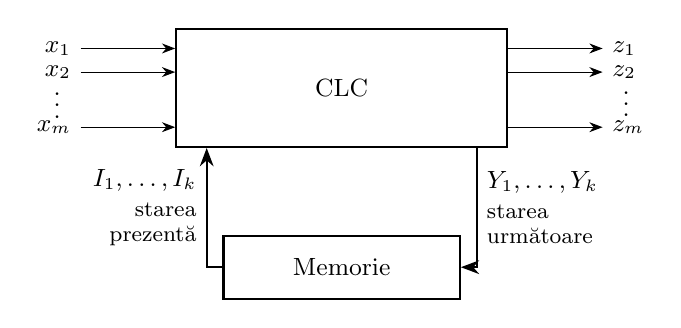
\begin{tikzpicture}[>=Stealth, font=\small,
  blk/.style={draw, thick, minimum width=4.2cm, minimum height=1.5cm}]
  \node[blk] (clc) {CLC};
  \node[blk, minimum width=3cm, minimum height=0.8cm, below=1.1cm of clc] (mem) {Memorie};

  % intrari
  \foreach \i/\lbl/\dy in {1/$x_1$/0.5, 2/$x_2$/0.2, 3/$x_m$/-0.5}{
    \draw[->] ($(clc.west)+(-1.2,\dy)$) node[left]{\lbl} -- ($(clc.west)+(0,\dy)$);
  }
  \node at ($(clc.west)+(-1.5,-0.12)$) {$\vdots$};
  % iesiri
  \foreach \i/\lbl/\dy in {1/$z_1$/0.5, 2/$z_2$/0.2, 3/$z_m$/-0.5}{
    \draw[->] ($(clc.east)+(0,\dy)$) -- ($(clc.east)+(1.2,\dy)$) node[right]{\lbl};
  }
  \node at ($(clc.east)+(1.5,-0.1)$) {$\vdots$};

  % stare urmatoare: CLC -> memorie (dreapta)
  \draw[->, thick] ($(clc.south east)+(-0.4,0)$) |- (mem.east)
     node[pos=0.25, right, align=left]{$Y_1,\dots,Y_k$\\ \footnotesize starea\\[-2pt]\footnotesize următoare};
  % stare prezenta: memorie -> CLC (stanga)
  \draw[->, thick] (mem.west) -| ($(clc.south west)+(0.4,0)$)
     node[pos=0.75, left, align=right]{$I_1,\dots,I_k$\\ \footnotesize starea\\[-2pt]\footnotesize prezentă};
\end{tikzpicture}
\end{center}

Un CLS este un circuit de prelucrare a informației discrete în care se pun în
evidență următoarele seturi de mărimi:
\begin{itemize}
  \item un set de variabile de intrare (externe): $X = \{x_1, x_2, x_3, \dots\}$;
  \item un set de variabile de ieșire: $Z = \{z_1, z_2, z_3, \dots\}$;
  \item un set de variabile de stare: $Y = \{y_1, y_2, y_3, \dots\}$.
\end{itemize}

Pentru semnalele de stare se folosește următoarea notație:
\begin{itemize}
  \item $Y_j\ (j=\overline{1,k})$ -- \textbf{funcții de excitație} sau
  \emph{variabile secundare de excitație}: sunt semnalele care intră în memorie
  și definesc \textbf{starea internă următoare} $(t+1)$;
  \item $I_j\ (j=\overline{1,k})$ -- \textbf{variabile secundare (de stare)}:
  sunt semnalele care ies din blocul de memorie și definesc
  \textbf{starea prezentă} $(t)$.
\end{itemize}

Cele $k$ variabile de stare definesc, prin valorile pe care le pot lua la
momentul $t$, starea internă $s_t$ a circuitului. Mulțimea stărilor interne
\[
  S = \{s_1, s_2, \dots, s_q\}
\]
în care se poate afla un circuit într-un interval de timp $T$ este
\textbf{finită}.

\section{Evoluția în timp și funcțiile caracteristice}

Dacă socotim că ne aflăm în \emph{Sistemul Automatelor Dinamice}, timpul nu
apare explicit în funcționarea circuitului; el apare însă în tranziția dintre
stările interne.

Dacă la momentul $t_i \in T$ se modifică cel puțin una dintre intrările $X$,
circuitul tranzitează într-o altă stare internă din mulțimea $S$, tranziția din
vechea în noua stare încheindu-se la momentul $t_i + \Delta t$ sau $t_i + 1$.
Tranziția în noua stare atrage după sine și modificarea ieșirilor circuitului, în
concordanță cu logica de control/reglare pentru care circuitul a fost proiectat.
Deci stările circuitului la momentul $t$ sunt definite de variabilele secundare
de stare, iar cele de la momentul $t+1$ de variabilele de excitație ale
circuitului.

În concluzie, orice circuit logic secvențial poate fi descris prin relații între
intrări, ieșiri, starea prezentă și starea următoare; astfel se pot scrie
următoarele seturi de relații:

\noindent pentru ieșiri:
\begin{equation}\label{eq:iesiri}
\left\{
\begin{aligned}
  z_1 &= g_1(x_1, \dots, x_m, I_1, \dots, I_k)\\
      &\ \ \vdots\\
  z_m &= g_m(x_1, \dots, x_m, I_1, \dots, I_k)
\end{aligned}
\right.
\end{equation}

\noindent pentru stările următoare:
\begin{equation}\label{eq:stari}
\left\{
\begin{aligned}
  Y_1 &= f_1(x_1, \dots, x_m, I_1, \dots, I_k)\\
      &\ \ \vdots\\
  Y_k &= f_k(x_1, \dots, x_m, I_1, \dots, I_k)
\end{aligned}
\right.
\end{equation}

Seturile de relații \eqref{eq:iesiri} și \eqref{eq:stari} reprezintă
explicitarea, pe de o parte, a funcțiilor de ieșire $g$, care stabilesc o relație
între intrările și stările la momentul $t$ și ieșirile la momentul $t$, iar pe de
altă parte explicitarea funcțiilor de tranziție $f$, care stabilesc o legătură
între intrările și stările prezente la $t$ și starea următoare la $t+1$.

\begin{retine}
Funcțiile $f$ și $g$ se numesc \textbf{funcții caracteristice} și definesc
complet evoluția unui circuit logic secvențial la orice moment de timp.
\end{retine}

Se consideră că orice CLS pe care îl studiem are o \textbf{comportare
deterministă}: pentru o anumită stare a intrărilor și o anumită stare internă
există o singură evoluție sau tranziție posibilă într-o stare internă următoare.

Funcțiile $g$ sunt realizate de rețeaua logică combinațională, iar funcțiile $f$
de tranziție sunt determinate atât de rețeaua logică combinațională, cât și de
blocul de memorie.

\section{Stări stabile și instabile}

\begin{itemize}
  \item O stare internă este \textbf{stabilă} dacă starea internă următoare este
  egală cu starea internă prezentă:
  \[
    Y_j = I_j \qquad (j = \overline{1,k}).
  \]
  O stare internă se menține stabilă până când se modifică cel puțin o intrare.

  \item O stare internă este \textbf{instabilă} dacă, într-o secvență dată și
  nemodificată a intrărilor, starea internă următoare diferă de starea internă
  prezentă prin cel puțin o variabilă de stare. În mod normal, un CLS se poate
  afla într-o stare internă instabilă doar un timp finit.
\end{itemize}

Un CLS are o comportare deterministă dacă pentru fiecare secvență a intrărilor
există cel puțin o stare internă stabilă.

\section{Modelul matematic general}

În concluzie, comportarea unui CLS este descrisă matematic printr-un
\textbf{cvintuplu}:
\begin{equation}\label{eq:cvintuplu}
  C = (X, Z, S, f, g)
\end{equation}
unde
\[
  f : X \times S \to S, \qquad g : X \times S \to Z .
\]

Un CLS se numește \textbf{cu stări finite} dacă mulțimile $X$, $Z$, $S$ sunt
finite (deci discrete), iar modelul lui matematic se numește
\textbf{automat finit}. Spațiul timpului, deși nu apare în definiție, este
discret și format din $\mathbb{N}$.

Un CLS poate fi definit matematic și printr-un \textbf{triplet}:
\begin{equation}\label{eq:triplet}
  C = (X, Z, M), \qquad M : X \to Z \quad \text{(relația intrare--ieșire)}.
\end{equation}
Această definiție este utilă în experimente și în diagnoza de sistem, în timp ce
definiția prin cvintuplu se folosește în analiza și sinteza circuitelor.

\begin{retine}
Rezultă că circuitele logice combinaționale reprezintă un \textbf{caz particular}
al celor secvențiale, în care $S = \varnothing$.
\end{retine}

\section{Automate Mealy și Moore}

CLS descrise prin \eqref{eq:iesiri}, \eqref{eq:stari} și \eqref{eq:cvintuplu}
se numesc de tipul \textbf{Mealy}.

Un caz particular al automatelor Mealy îl reprezintă CLS de tip
\textbf{Moore}. La acest tip, modelul matematic este tot un cvintuplu, dar
ieșirile depind doar de starea internă:
\begin{equation}\label{eq:moore}
\left\{
\begin{aligned}
  z_1 &= g_1(I_1, \dots, I_k)\\
      &\ \ \vdots\\
  z_m &= g_m(I_1, \dots, I_k)
\end{aligned}
\right.
\qquad\qquad g : S \to Z .
\end{equation}

Matematic se poate demonstra că cele două modele sunt \textbf{echivalente} și
există algoritmi pentru conversie.

\section{Clasificarea CLS}

\subsection{După modul de construcție și funcționare}

În funcție de modul de construcție și de funcționare, CLS pot fi:
\begin{itemize}
  \item \textbf{asincrone} (CLSA);
  \item \textbf{sincrone} (CLSS).
\end{itemize}

La \textbf{CLSA}, tranzițiile între stări au loc la momente arbitrare de timp,
determinate de întârzierile inerente apărute în transmiterea semnalelor pe căile
de reacție:
\[
  \text{starea internă următoare} \;\to\; \text{starea internă prezentă}.
\]

La \textbf{CLSS}, tranzițiile în stările următoare se fac la momente bine
precizate de timp, marcate prin impulsul de tact/ceas.

CLSA sunt mai simple din punct de vedere constructiv și se pretează la automatizări
mai puțin complexe. Ele prezintă însă un dezavantaj important: întârzierile care
apar în transmiterea semnalelor pe căile de reacție, fiind diferite, pot face să
apară un fenomen de \emph{hazard} sau \emph{concurs}, numit și \emph{de tranziție}.

\subsection{După elementele din componența buclei de reacție}

\begin{itemize}
  \item \textbf{CLS cu reacții directe}, la care funcția de memorare este
  determinată de întârzierile care apar pe bucla de reacție;
  \item \textbf{CLS cu reacții prin celule de întârziere}, care au rolul unei
  memorii tampon;
  \item \textbf{CLS cu reacții prin celule de memorie binare propriu-zise}
  (crearea unei memorii permanente).
\end{itemize}

CLS din prima categorie sunt mereu \textbf{asincrone}, iar celelalte pot fi atât
asincrone, cât și sincrone.


\end{document}
